\documentclass[12pt, a4paper]{article}

% ─── Packages ──────────────────────────────────────────────────────────────────
\usepackage[a4paper, margin=2.5cm, headheight=24pt]{geometry}
\usepackage{xcolor}
\usepackage{titlesec}
\usepackage{booktabs}
\usepackage{longtable}
\usepackage{array}
\usepackage{enumitem}
\usepackage{hyperref}
\usepackage{fancyhdr}
\usepackage{parskip}
\usepackage{colortbl}
\usepackage{multirow}
\usepackage[T1]{fontenc}
\usepackage[utf8]{inputenc}


\usepackage{tocloft}
\usepackage{tikz}
\usepackage{tabularx}
\usepackage{makecell}
\usepackage{boldline}
\usepackage{graphicx}
\usepackage{pdfpages}

% ─── Colors ────────────────────────────────────────────────────────────────────
\definecolor{pharmagreen}{HTML}{2D6A4F}
\definecolor{darkgreen}{HTML}{1A3C2E}
\definecolor{lightgreen}{HTML}{D8F3DC}
\definecolor{medgreen}{HTML}{B7E4C7}
\definecolor{rowgray}{HTML}{F4F4F4}
\definecolor{textgray}{HTML}{555555}
\definecolor{darktext}{HTML}{1B1B1B}
\definecolor{winfill}{HTML}{C8F5DA}
\definecolor{winborder}{HTML}{2D6A4F}
\definecolor{pharmaorange}{HTML}{E07B39}
\definecolor{lightorange}{HTML}{FFF0E6}
\definecolor{midorange}{HTML}{FDDCC8}

% ─── Hyperref ──────────────────────────────────────────────────────────────────
\hypersetup{
  colorlinks=true,
  linkcolor=pharmagreen,
  urlcolor=pharmagreen,
  pdftitle={PharmaZen SDLC Selection},
  pdfauthor={Zunayed Iqbal Shaed, Rudro Roy, Ovizit Dutt, Tasnim Rashid Medha}
}

% ─── Section Formatting ────────────────────────────────────────────────────────
\titleformat{\section}
  {\color{pharmagreen}\Large\bfseries}{\thesection}{1em}{}
  [\color{pharmagreen}\titlerule]
\titleformat{\subsection}
  {\color{darkgreen}\large\bfseries}{\thesubsection}{1em}{}
\titleformat{\subsubsection}
  {\color{pharmagreen}\normalsize\bfseries}{\thesubsubsection}{1em}{}
\titlespacing*{\section}{0pt}{20pt}{8pt}
\titlespacing*{\subsection}{0pt}{14pt}{6pt}
\titlespacing*{\subsubsection}{0pt}{10pt}{4pt}

% ─── Header & Footer ───────────────────────────────────────────────────────────
\pagestyle{fancy}
\fancyhf{}
\fancyhead[L]{\small\color{pharmagreen}\textbf{PharmaZen}
  \color{textgray} SDLC Selection}
\fancyhead[R]{\small\color{textgray}SE Lab Report}
\fancyfoot[C]{\small\color{textgray}PharmaZen --- SDLC Selection \quad|\quad Page \thepage}
\renewcommand{\headrulewidth}{0.4pt}
\renewcommand{\headrule}{\hbox to\headwidth{%
  \color{pharmagreen}\leaders\hrule height \headrulewidth\hfill}}
\renewcommand{\footrulewidth}{0.4pt}
\renewcommand{\footrule}{\hbox to\headwidth{%
  \color{pharmagreen}\leaders\hrule height \footrulewidth\hfill}}

% ─── Column Types ──────────────────────────────────────────────────────────────
\newcolumntype{L}[1]{>{\raggedright\arraybackslash}p{#1}}
\newcolumntype{C}[1]{>{\centering\arraybackslash}p{#1}}

% ─── Section Badge ─────────────────────────────────────────────────────────────
\newcommand{\sectionbadge}[2]{%
  \vspace{12pt}\noindent
  \colorbox{pharmagreen}{%
    \parbox{\dimexpr\textwidth-2\fboxsep\relax}{%
      \vspace{4pt}
      \color{white}\small\bfseries\MakeUppercase{Section #1 \quad·\quad #2}
      \vspace{4pt}
    }%
  }\vspace{6pt}
}

% ══════════════════════════════════════════════════════════════════════════════
\begin{document}
\pagenumbering{gobble}

% ─── COVER ────────────────────────────────────────────────────────────────────
\begin{titlepage}
  \centering
  \vspace*{2.5cm}
  {\fontsize{40}{48}\selectfont\color{pharmagreen}\textbf{PharmaZen}}\\[0.4cm]
  {\large\color{textgray} Online Pharmacy \& Health Products Platform}
  \vspace{1.4cm}

  
\begin{tikzpicture}
    \draw[color=pharmagreen, line width=1.5pt] (0,0) -- (\textwidth,0);
  \end{tikzpicture}
  \vspace{0.5cm}

  {\Large\color{darkgreen}\textbf{SDLC Model Selection}}\\[0.3cm]
  {\normalsize\color{textgray} Software Development Life Cycle Analysis \& Justification}
  \vspace{0.5cm}

  \begin{tikzpicture}
    \draw[color=pharmagreen, line width=0.6pt] (0,0) -- (\textwidth,0);
  \end{tikzpicture}
  \vspace{1.6cm}

  \colorbox{lightgreen}{%
    \parbox{13cm}{%
      \vspace{12pt}\centering
      \renewcommand{\arraystretch}{1.7}
      \begin{tabular}{rl}
        \textbf{Project:}       & PharmaZen --- Online Pharmacy Platform \\
        \textbf{Course:}        & SE (Software Engineering) \\
        \textbf{Date:}          & March 2026 \\[4pt]
        \textbf{Team Members:}  & Zunayed Iqbal Shaed \quad\quad   (23524202028) \\
                                & Rudro Roy \quad\quad\quad\quad\quad\quad\;\;  (23524202060) \\
                                & Tasnim Rashid Medha \quad\quad (23524202088) \\
                                & Ovizit Dutt Ovi \quad\quad\quad\quad\quad (23524202118) \\
      \end{tabular}
      \vspace{12pt}
    }%
  }

  \vfill
  
\begin{tikzpicture}
    \draw[color=pharmagreen, line width=1.5pt] (0,0) -- (\textwidth,0);
  \end{tikzpicture}
  \vspace{0.4cm}
  {\small\color{textgray}Bangladesh University of Professionals \quad|\quad Department of Computer Science \& Engineering}
\end{titlepage}

\pagenumbering{roman}
\tableofcontents
\newpage
\pagenumbering{arabic}

% ══════════════════════════════════════════════════════════════════════════════
%  SECTION 3 — SDLC
% ══════════════════════════════════════════════════════════════════════════════
\sectionbadge{3}{SDLC}
\section{SDLC}

Software Development Life Cycle (SDLC) is a structured process used to design, develop, test, and deploy software systems efficiently and with high quality. The life cycle defines a methodology for improving the quality of software and the overall development process.

A typical Software Development Life Cycle consists of the following stages:

\begin{itemize}[leftmargin=1.5em, itemsep=5pt]
  \item \textbf{\underline{Stage 1: Planning and Requirement Analysis}} ---
        The most fundamental stage, performed by the senior members of the team with inputs from the customer, market surveys, and domain experts. This stage covers project feasibility, risk identification, and quality assurance planning.

  \item \textbf{\underline{Stage 2: Defining Requirements}} ---
        Clearly define and document the product requirements and get them approved. This is done through an SRS (Software Requirement Specification) document which consists of all the product requirements to be designed and developed during the project life cycle.

  \item \textbf{\underline{Stage 3: Designing the Product Architecture}} ---
        The SRS serves as a reference for architects to develop the best architecture. A DDS (Design Document Specification) documents one or more proposed approaches. The best approach is selected based on risk, robustness, budget, and time constraints.

  \item \textbf{\underline{Stage 4: Building or Developing the Product}} ---
        Actual development starts and the product is built. Programming code is generated as per DDS. Developers follow coding guidelines and use tools such as compilers, debuggers, and version control systems.

  \item \textbf{\underline{Stage 5: Testing the Product}} ---
        Product defects are reported, tracked, fixed, and retested until the product reaches the quality standards defined in the SRS.

  \item \textbf{\underline{Stage 6: Deployment in the Market and Maintenance}} ---
        The product is formally released and deployed. Maintenance is carried out for the existing customer base, addressing bugs, security patches, and performance improvements.
\end{itemize}

% ─────────────────────────────────────────────────────────────────────────────
\subsection{Common SDLC Models}

\vspace{6pt}
\renewcommand{\arraystretch}{1.5}
\begin{tabular}{|L{2.8cm}|L{4.5cm}|L{7.5cm}|}
  \hline
  \rowcolor{pharmagreen}
  \textbf{\color{white}Model} &
  \textbf{\color{white}Approach} &
  \textbf{\color{white}Best Suited For} \\
  \hline
  \rowcolor{lightgreen}\textbf{Waterfall} & Sequential, phase-by-phase & Projects with stable, well-documented requirements and fixed scope \\
  \hline
  \rowcolor{rowgray}\textbf{V-Model} & Extension of Waterfall with parallel testing at each stage & Safety-critical systems requiring rigorous validation \\
  \hline
  \rowcolor{lightgreen}\textbf{Iterative} & Development in repeated cycles & Projects where requirements are expected to evolve over time \\
  \hline
  \rowcolor{rowgray}\textbf{Incremental} & System built in parts (increments) & Systems needing early partial delivery \\
  \hline
  \rowcolor{lightgreen}\textbf{Spiral} & Iterative development with risk analysis at each loop & Large, high-risk, and complex enterprise projects \\
  \hline
  \rowcolor{rowgray}\textbf{Agile} & Flexible, sprint-based, continuous feedback & Dynamic requirements with high client involvement \\
  \hline
\end{tabular}

% ─────────────────────────────────────────────────────────────────────────────
\subsection{Factors for SDLC Selection}

When selecting an SDLC model, the following factors must be considered:

\begin{itemize}[leftmargin=1.5em, itemsep=4pt]
  \item \textbf{Project size} --- small / medium / large
  \item \textbf{Requirement clarity} --- clear and fixed vs.\ frequently changing
  \item \textbf{Risk level} --- low, medium, or high tolerance for uncertainty
  \item \textbf{Time constraints} --- strict deadline or flexible schedule
  \item \textbf{Budget} --- fixed budget vs.\ flexible funding
  \item \textbf{Customer involvement} --- high involvement or minimal
  \item \textbf{Team expertise} --- familiarity with specific models or processes
\end{itemize}

\newpage
% ══════════════════════════════════════════════════════════════════════════════
%  SECTION 4 — METHODOLOGY
% ══════════════════════════════════════════════════════════════════════════════
\sectionbadge{4}{Methodology}
\section{Methodology}

The following five-step methodology was applied to select the most suitable SDLC model for the PharmaZen project.

% ─────────────────────────────────────────────────────────────────────────────
\subsection*{\textit{Step 1: Analyze the Problem}}
\addcontentsline{toc}{subsection}{Step 1: Analyze the Problem}

PharmaZen is a full-stack e-commerce web application for pharmaceutical and health products targeting the Bangladesh market. The problem analysis identified the following:

\begin{itemize}[leftmargin=1.5em, itemsep=4pt]
  \item \textbf{System requirements:} Comprehensive functional requirements covering user authentication, product catalog, prescription management, payment integration (mock bKash as it is not a real business app), order management, and admin dashboard — all fully documented in the SRS.
  \item \textbf{Project scope:} Clearly bounded and fixed for v1.0 — a single-country web platform with no native mobile app; deployed on Vercel with a PostgreSQL database on Neon Tech.
  \item \textbf{User needs:} Customers need a trustworthy online pharmacy; pharmacists need a workflow for prescription verification; administrators need full platform control via a dashboard.
\end{itemize}

% ─────────────────────────────────────────────────────────────────────────────
\subsection*{\textit{Step 2: Evaluate Project Characteristics}}
\addcontentsline{toc}{subsection}{Step 2: Evaluate Project Characteristics}

\vspace{6pt}
\renewcommand{\arraystretch}{1.5}
\begin{tabular}{|L{4.5cm}|L{10.5cm}|}
  \hline
  \rowcolor{pharmagreen}\textbf{\color{white}Characteristic} & \textbf{\color{white}PharmaZen Assessment} \\
  \hline
  \rowcolor{lightgreen}\textbf{Requirement Stability} & Requirements are fully defined and documented in the SRS before development begins. No scope changes are anticipated. \\
  \hline
  \rowcolor{rowgray}\textbf{Risk Level} & Low to medium. Technology stack (React, Node.js, PostgreSQL, Vercel) is well-established. Payment mock server reduces real-world financial risk. \\
  \hline
  \rowcolor{lightgreen}\textbf{Complexity} & Medium. Multiple integrated modules (auth, catalog, prescriptions, payments, orders, admin) but well-scoped with clear boundaries. \\
  \hline
  \rowcolor{rowgray}\textbf{Delivery Timeline} & Sufficient time allocated across 10 weeks with distinct phases for planning, design, development, testing, and deployment. \\
  \hline
\end{tabular}

% ─────────────────────────────────────────────────────────────────────────────
\subsection*{\textit{Step 3: Compare SDLC Models}}
\addcontentsline{toc}{subsection}{Step 3: Compare SDLC Models}

A comparison was made across all major SDLC models against project-specific criteria. Refer to Section 5 for the full scored comparison matrix.

% ─────────────────────────────────────────────────────────────────────────────
\subsection*{\textit{Step 4: Select Suitable Model}}
\addcontentsline{toc}{subsection}{Step 4: Select Suitable Model}

Based on the project characteristics and the scored model matrix in Section 5, the \textbf{Waterfall Model} was selected as the most suitable SDLC for PharmaZen.

% ─────────────────────────────────────────────────────────────────────────────
\subsection*{\textit{Step 5: Justify Selection}}
\addcontentsline{toc}{subsection}{Step 5: Justify Selection}

The Waterfall model fits PharmaZen because:
\begin{itemize}[leftmargin=1.5em, itemsep=4pt]
  \item All functional requirements are well-defined and stable — the hallmark condition for Waterfall suitability
  \item The project has a fixed scope, fixed timeline (10 weeks), and a small fixed team of three members
  \item Sequential phases (Planning $\rightarrow$ Design $\rightarrow$ Frontend Dev $\rightarrow$ Backend Dev $\rightarrow$ Testing $\rightarrow$ Deployment) align naturally with the project's structure
  \item A dedicated testing phase is explicitly included before Vercel deployment
  \item The technology stack is well-known to the team, reducing the need for iterative prototyping
  \item Deployment is to a single target environment (Vercel + Neon Tech), requiring no phased rollout strategy
\end{itemize}

\newpage
% ══════════════════════════════════════════════════════════════════════════════
%  SECTION 5 — SDLC MODEL SELECTION FOR PHARMAZEN
% ══════════════════════════════════════════════════════════════════════════════
\sectionbadge{5}{SDLC Model Selection for PharmaZen}
\section{SDLC Model Selection for PharmaZen}

A comparative analysis of SDLC models was conducted for the PharmaZen project based on seven project-specific criteria. Each criterion was assigned a priority weight (1 = Low, 2 = Medium, 3 = High) reflecting its importance to the project. Each model was then scored against each criterion (1 = Poor fit, 2 = Partial fit, 3 = Strong fit), and a weighted score was calculated as: \textbf{Weighted Score = Priority $\times$ Model Score}.

% ─────────────────────────────────────────────────────────────────────────────
\subsection{Model Comparison Matrix}

\vspace{8pt}
\renewcommand{\arraystretch}{1.6}
\setlength{\tabcolsep}{5pt}

\begin{longtable}{|L{4.0cm}|C{0.8cm}|C{1.5cm}|C{1.3cm}|C{1.5cm}|C{1.6cm}|C{1.2cm}|C{1.2cm}|}
  \hline
  \rowcolor{pharmagreen}
  \textbf{\color{white}\small Criteria} &
  \textbf{\color{white}\small Pri.} &
  \textbf{\color{white}\small Water-fall} &
  \textbf{\color{white}\small V-Model} &
  \textbf{\color{white}\small Iterative} &
  \textbf{\color{white}\small Incremental} &
  \textbf{\color{white}\small Spiral} &
  \textbf{\color{white}\small Agile} \\
  \hline
  \endfirsthead
  \hline
  \rowcolor{pharmagreen}
  \textbf{\color{white}\small Criteria} &
  \textbf{\color{white}\small Pri.} &
  \textbf{\color{white}\small Water-fall} &
  \textbf{\color{white}\small V-Model} &
  \textbf{\color{white}\small Iterative} &
  \textbf{\color{white}\small Incremental} &
  \textbf{\color{white}\small Spiral} &
  \textbf{\color{white}\small Agile} \\
  \hline
  \endhead

  \rowcolor{lightgreen}
  \small Well-defined \& stable requirements &
  \small 3 & \small 3×3=\textbf{9} & \small 3×3=\textbf{9} & \small 1×3=\textbf{3} & \small 2×3=\textbf{6} & \small 2×3=\textbf{6} & \small 1×3=\textbf{3} \\
  \hline

  \rowcolor{rowgray}
  \small Fixed project scope (v1.0) &
  \small 3 & \small 3×3=\textbf{9} & \small 3×3=\textbf{9} & \small 1×3=\textbf{3} & \small 2×3=\textbf{6} & \small 2×3=\textbf{6} & \small 1×3=\textbf{3} \\
  \hline

  \rowcolor{lightgreen}
  \small Sequential phases fit timeline &
  \small 2 & \small 3×2=\textbf{6} & \small 2×2=\textbf{4} & \small 2×2=\textbf{4} & \small 2×2=\textbf{4} & \small 2×2=\textbf{4} & \small 2×2=\textbf{4} \\
  \hline

  \rowcolor{rowgray}
  \small Dedicated testing phase &
  \small 3 & \small 3×3=\textbf{9} & \small 3×3=\textbf{9} & \small 2×3=\textbf{6} & \small 2×3=\textbf{6} & \small 2×3=\textbf{6} & \small 3×3=\textbf{9} \\
  \hline

  \rowcolor{lightgreen}
  \small Clear documentation output &
  \small 3 & \small 3×3=\textbf{9} & \small 3×3=\textbf{9} & \small 2×3=\textbf{6} & \small 2×3=\textbf{6} & \small 2×3=\textbf{6} & \small 1×3=\textbf{3} \\
  \hline

  \rowcolor{rowgray}
  \small Low-risk, small team project &
  \small 2 & \small 3×2=\textbf{6} & \small 2×2=\textbf{4} & \small 2×2=\textbf{4} & \small 2×2=\textbf{4} & \small 1×2=\textbf{2} & \small 2×2=\textbf{4} \\
  \hline

  \rowcolor{lightgreen}
  \small Single deployment target (Vercel + Neon) &
  \small 2 & \small 3×2=\textbf{6} & \small 2×2=\textbf{4} & \small 2×2=\textbf{4} & \small 3×2=\textbf{6} & \small 2×2=\textbf{4} & \small 2×2=\textbf{4} \\
  \hline

  \rowcolor{winfill}
  \textbf{\small Total Weighted Score} &
  \textbf{---} &
  \textbf{\color{pharmagreen}54} &
  \textbf{48} &
  \textbf{30} &
  \textbf{38} &
  \textbf{34} &
  \textbf{30} \\
  \hline
\end{longtable}

\noindent\small\textit{Priority: 3 = High, 2 = Medium, 1 = Low. \quad Model Score: 3 = Strong fit, 2 = Partial fit, 1 = Poor fit.}

% ─────────────────────────────────────────────────────────────────────────────
\subsection{Justification}

The scoring results are summarized below:

\vspace{6pt}
\renewcommand{\arraystretch}{1.5}
\begin{tabular}{|L{3.8cm}|C{2.5cm}|L{8.5cm}|}
  \hline
  \rowcolor{pharmagreen}\textbf{\color{white}Model} & \textbf{\color{white}Score} & \textbf{\color{white}Verdict} \\
  \hline
  \rowcolor{winfill}\textbf{Waterfall} & \textbf{\color{pharmagreen}54} & \textbf{Selected --- Highest score; best fits PharmaZen's stable requirements and fixed scope} \\
  \hline
  \rowcolor{rowgray}V-Model & 48 & Strong on testing but adds unnecessary overhead for a student project \\
  \hline
  Incremental & 38 & Useful for partial delivery, but PharmaZen targets a single full release \\
  \hline
  \rowcolor{rowgray}Spiral & 34 & Overkill risk management for a low-risk, well-scoped project \\
  \hline
  Iterative & 30 & Suited for evolving requirements; PharmaZen requirements are already fixed \\
  \hline
  \rowcolor{rowgray}Agile & 30 & Requires continuous client feedback loops; not aligned with a fixed-scope academic project \\
  \hline
\end{tabular}

\vspace{12pt}
\noindent\textbf{Conclusion:} The \textbf{Waterfall Model} achieved the highest weighted score of \textbf{54}, making it the most suitable SDLC for PharmaZen. The key justifications are:

\begin{itemize}[leftmargin=1.5em, itemsep=5pt]
  \item \textbf{Stable, fully documented requirements:} The SRS was completed before development began. All 21 functional requirements and 14 non-functional requirements are clearly specified, which is the primary precondition for Waterfall's success.
  \item \textbf{Fixed scope and timeline:} PharmaZen v1.0 targets a clearly bounded feature set across a 10-week schedule with no planned scope changes.
  \item \textbf{Sequential phase alignment:} The natural project breakdown — Planning $\rightarrow$ UI/UX Design $\rightarrow$ Frontend Development $\rightarrow$ Backend Development \& Database Integration $\rightarrow$ Testing $\rightarrow$ Vercel Deployment — maps directly onto the Waterfall phase sequence.
  \item \textbf{Dedicated testing phase:} A full week is allocated exclusively for testing and debugging before deployment, which Waterfall explicitly supports.
  \item \textbf{Single, well-defined deployment target:} The platform deploys to Vercel (frontend + serverless API) with PostgreSQL on Neon Tech — a single, known target environment requiring no phased or multi-environment rollout.
  \item \textbf{Small, expert team:} A three-member team with clearly assigned roles (Project Manager/Backend Lead, Frontend/UI/UX, Backend/API) works most efficiently with a structured sequential model rather than sprint-based approaches.
\end{itemize}

\newpage
% ══════════════════════════════════════════════════════════════════════════════
%  SECTION 6 — UML
% ══════════════════════════════════════════════════════════════════════════════
\sectionbadge{6}{UML}
\section{UML}

Unified Modeling Language (UML) provides a standardised way to visualise the design of a system. For PharmaZen, the primary UML artefact produced at this stage is a \textbf{Use Case Diagram}, which captures the functional scope of the platform by depicting the interactions between the system's actors and the use cases it supports.
% ─────────────────────────────────────────────────────────────────────────────
\vspace{10pt}
\noindent
\begin{center}
  \fbox{%
    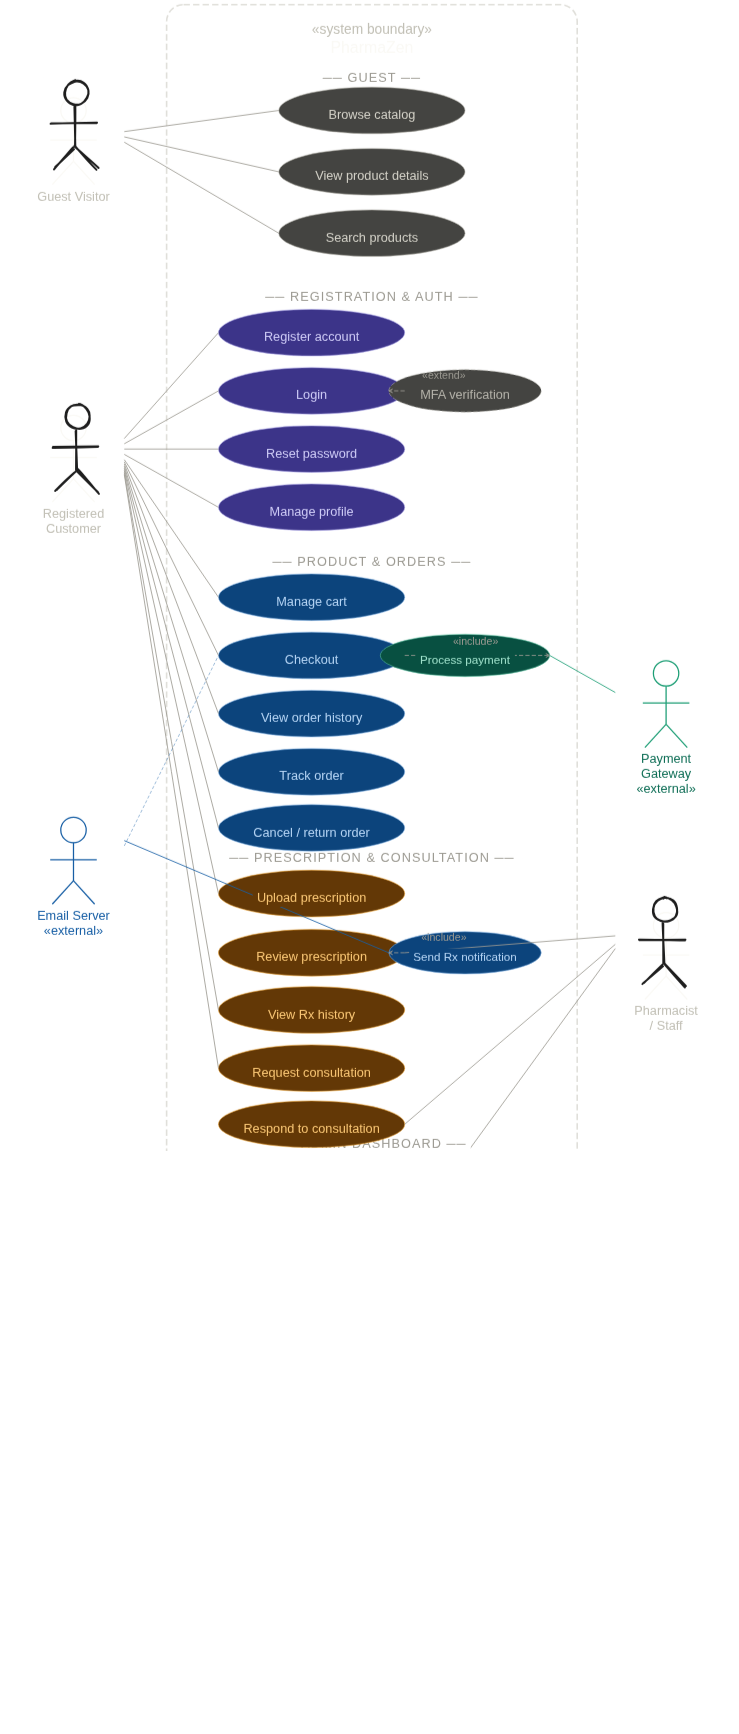
\includegraphics[width=0.92\textwidth, keepaspectratio]{pharmazen_diagram1.png}%
  }
  \fbox{%
    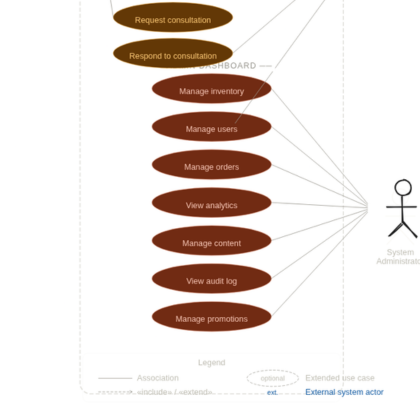
\includegraphics[width=0.92\textwidth, keepaspectratio]{pharmazen_diagram2.png}%
  }
\end{center}
\vspace{6pt}
\begin{center}
  \small\textit{Figure 6.1 --- PharmaZen UML Use Case Diagram}
\end{center}

% ─────────────────────────────────────────────────────────────────────────────
\newpage
\subsection{Use Case Description Table}

The table below provides a structured description of each use case identified in the diagram. The \textit{Included / Extends} column notes any \texttt{«include»} or \texttt{«extend»} relationships present in the diagram.

\vspace{8pt}
\renewcommand{\arraystretch}{1.55}
\setlength{\tabcolsep}{5pt}

\begin{longtable}{|C{0.8cm}|L{2.4cm}|L{3.0cm}|L{3.2cm}|L{5.8cm}|}
  \hline
  \rowcolor{pharmagreen}
  \textbf{\color{white}\small Sl.} &
  \textbf{\color{white}\small Use Case} &
  \textbf{\color{white}\small Primary Actor} &
  \textbf{\color{white}\small Included / Extends} &
  \textbf{\color{white}\small Brief Description} \\
  \hline
  \endfirsthead
  \hline
  \rowcolor{pharmagreen}
  \textbf{\color{white}\small Sl.} &
  \textbf{\color{white}\small Use Case} &
  \textbf{\color{white}\small Primary Actor} &
  \textbf{\color{white}\small Included / Extends} &
  \textbf{\color{white}\small Brief Description} \\
  \hline
  \endhead

  \rowcolor{lightorange}
  \small UC-01 &
  \small Browse Catalog &
  \small Guest Visitor &
  \small --- &
  \small Any unauthenticated visitor can browse the product catalog, view product details, and search or filter items without logging in. \\
  \hline

  \rowcolor{rowgray}
  \small UC-02 &
  \small Register Account &
  \small Guest Visitor &
  \small --- &
  \small A new user provides personal details (name, email, password, phone) to create a PharmaZen account and gain access to customer-only features. \\
  \hline

  \rowcolor{lightorange}
  \small UC-03 &
  \small Login &
  \small Registered Customer &
  \small --- &
  \small An existing user authenticates with their email and password to access their personalised dashboard, orders, and prescription history. \\
  \hline

  \rowcolor{lightorange}
  \small UC-04 &
  \small Manage Cart &
  \small Registered Customer &
  \small --- &
  \small An authenticated customer adds products to, removes products from, and updates quantities in their shopping cart prior to checkout. \\
  \hline

  \rowcolor{rowgray}
  \small UC-06 &
  \small Checkout &
  \small Registered Customer &
  \small \texttt{«include»} Process Payment &
  \small The customer reviews their cart, selects a delivery address, and confirms the order. Checkout mandatorily triggers the Process Payment use case. \\
  \hline

  \rowcolor{lightorange}
  \small UC-07 &
  \small Process Payment &
  \small Registered Customer &
  \small \texttt{«include»} in Checkout; Payment Gateway (external) &
  \small The system processes the transaction via the mock bKash Payment Gateway. On success the order is confirmed; on failure the user is notified. \\
  \hline

  \rowcolor{rowgray}
  \small UC-08 &
  \small Upload Prescription &
  \small Registered Customer &
  \small --- &
  \small A customer uploads a scanned or photographed prescription for products requiring one. \\
  \hline

  \rowcolor{lightorange}
  \small UC-09 &
  \small Review Prescription &
  \small Pharmacist / Staff &
  \small --- &
  \small A pharmacist reviews uploaded prescriptions, verifies their validity, and either approves or rejects them. \\
  \hline

  \rowcolor{rowgray}
  \small UC-10 &
  \small Track Order &
  \small Registered Customer &
  \small --- &
  \small A logged-in customer views the real-time status of their placed orders (pending, processing, dispatched, delivered) from their order history page. \\
  \hline

  \rowcolor{rowgray}
  \small UC-11 &
  \small Manage Inventory &
  \small System Administrator &
  \small --- &
  \small The administrator adds new products, updates stock levels and pricing, removes discontinued items, and sets reorder thresholds via the admin dashboard. \\
  \hline

  \rowcolor{lightorange}
  \small UC-12 &
  \small Manage Users &
  \small System Administrator &
  \small --- &
  \small The administrator views, edits, activates, deactivates, or deletes registered user accounts and manages role assignments (Customer, Staff, Admin). \\
  \hline

  \rowcolor{rowgray}
  \small UC-13 &
  \small View Analytics &
  \small System Administrator &
  \small --- &
  \small The administrator views sales breakdown by medicine, generic name, company, and category through the analytics dashboard. \\
  \hline

\end{longtable}

% ─── DOCUMENT CONTROL ─────────────────────────────────────────────────────────
\newpage
{\color{pharmagreen}\large\bfseries Document Information}
\vspace{4pt}
\textcolor{pharmagreen}{\rule{\textwidth}{1pt}}
\vspace{8pt}

\renewcommand{\arraystretch}{1.5}
\begin{tabular}{|L{3.8cm}|L{11.2cm}|}
  \hline
  \rowcolor{lightgreen}\textbf{\small\color{darkgreen}Document Title} & \small PharmaZen --- SDLC Model Selection \& Use Case Analysis \\
  \hline
  \rowcolor{medgreen}\textbf{\small\color{darkgreen}Version} & \small 1.0 \\
  \hline
  \rowcolor{lightgreen}\textbf{\small\color{darkgreen}Submitted By} & \small Zunayed Iqbal Shaed (23524202028), Rudro Roy (23524202060), Ovizit Dutt (23524202118) \\
  \hline
  \rowcolor{medgreen}\textbf{\small\color{darkgreen}Date} & \small March 2026 \\
  \hline
  \rowcolor{lightgreen}\textbf{\small\color{darkgreen}Course} & \small SE (Software Engineering) \\
  \hline
  \rowcolor{medgreen}\textbf{\small\color{darkgreen}Selected SDLC Model} & \small Waterfall Model (Score: 54/54 max) \\
  \hline
\end{tabular}

\end{document}